

\chapter{Acustica e audio digitale}

\section{L' acustica e il suono}

L'acustica \`e quella branca della fisica che studia il suono, le sue cause, la sua propagazione e la sua ricezione.
La percezione sonora \`e normalmente legata alle vibrazioni del timpano nell'orecchio. 
Queste vibrazioni sono provocate da piccole variazioni di pressione nell'aria. 
La variazione di pressione dell'aria \`e quindi l'equivalente fisico del suono \cite{EAP}.
La vibrazione provoca una successione di compressioni e rarefazioni nel mezzo dell'ambiente circostante e tale disturbo comincia a propagarsi lontano dalla sorgente in tutte le direzioni (un caso visibile \`e quello delle onde sull'acqua). 
L'effetto uditivo, consiste nella percezione da parte di un apposito dispositivo (orecchio di esseri viventi o microfoni artificiali) delle piccole e rapidissime vibrazioni emesse appunto da una "sorgente sonora".

\section{Onde sonore}
La natura fisica del suono \`e di tipo ondulatorio, ovvero descrive un movimento che pu\`o essere rappresentato tramite un onda. 
Si tratta di onde meccaniche che trasportano energia lontano dalla sorgente sonora.
Alcune principali grandezze delle onde sono \cite{SELET}:
   \begin{description}
      \item[Periodo.] 
	Il periodo, o durata dell'oscillazione rappresenta il tempo in cui l'onda compie un'oscillazione e torna alla condizione iniziale.  
      \item[Frequenza.]
	La frequenza di un onda indica il numero di cicli completi che compie in un secondo:
	\[
	  f = \frac{1}{t}
	\]
	dove $f$ \`e la frequenza e $t$ \`e il periodo.
	In generale la frequenza di un evento si misura in $Hz$. 
	Ricordiamo che un $Hz$ \`e il numero di eventi che accadono in un secondo. 
      \item[Ampiezza.]
      L'ampiezza o intensit\`a invece \`e il valore massimo raggiunto dall'oscillazione stessa durante un periodo ed \`e determinata dalla quantit\`a di energia impiegata. 
      Viene espressa tramite i decibel.
      \item[Forma.]
	La forma dell'oscillazione \`e determinata dal numero delle componenti parziali e dal loro rapporto di frequenza, ampiezza e  fase. 
	Essa rappresenta l'aspetto dell'onda in base all'ampiezza e al tempo servendosi di coordinate cartesiane. 
    \end{description}
    
\begin{figure}[h!]
 \centering
 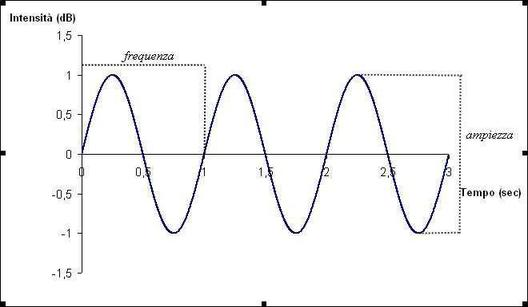
\includegraphics[width=0.5\textwidth]{./OndaSonora.jpg}
 % envelope.png: 220x138 pixel, 96dpi, 5.82x3.65 cm, bb=0 0 165 104
  \label{OndaSonora}
\caption{Rappresentazione delle principali grandezze dell'onda sonora \cite{IONDASON}}
\end{figure}



\section{Suono analogico e digitale}

Il suono \`e un flusso informativo di natura temporale che scorre all'interno di apparecchiature elettroniche. 
Questa informazione pu\`o essere rappresentata in due forme: analogico e digitale. 
Una rappresentazione analogica \`e una rappresentazione o trasformazione di una grandezza fisica tramite una sua analogia: in altre parole, si intende un sistema in cui una quantit\`a fisica continuamente variabile viene rappresentata da un'altra (ad esempio, la tensione di un segnale elettrico) nel modo pi\`u fedele possibile. 
La curva continua nel tempo delle variazioni di ampiezza viene rappresentata da una curva continua nel tempo delle variazioni di tensione elettrica. 


Una rappresentazione digitale non cerca di imitare la curva continua di ampiezza con una curva analoga ad essa, ma piuttosto assegna dei numeri che rappresentano di volta in volta il valore dell'ampiezza in istanti successivi di tempo. 
Sar\`a la successione di numeri a rappresentare l'andamento della curva. 
La rappresentazione digitale non \`e continua, ma discreta; cio\`e esistono degli eventi ben definiti che sono i valori dell'ampiezza in precisi istanti di tempo. 
I vantaggi della rappresentazione digitale e cio\`e di un codice simbolico sono molti: dalle operazioni di copia del segnale, a quelle di manipolazione. 
Ma un aspetto totalmente nuovo \`e la possibilit\`a di correzione degli errori introdotti dai supporti per la memorizzazione. 
Per errore si intende che alcuni numeri che rappresentano il segnale vengono letti in maniera differente da come era stati memorizzati o trasmessi.

\subsection{Discretizzazione}
Per sottoporre un segnale analogico ad elaborazioni digitali \`e necessario prima convertirlo in una sequenza di dati binari, ottenuti tramite due operazioni di discretizzazione: una discretizzazione nel dominio del tempo o campionamento che riduce gli infiniti valori di un segnale analogico in sequenze di campioni discreti e una discretizzazione nel dominio delle ampiezze o quantizzazione (del livello) che permette di rappresentare ciascun campione con un numero finito di bit. 
La necessit\`a di elaborare il segnale in forma digitale porta a limitare il numero delle informazioni e quindi a misurare le grandezze solo a valori discreti del tempo, attribuendo loro un certo numero discreto di valori, variabili fra un massimo e un minimo. 
I segnali acquisiti diventano quindi serie di valori corrispondenti agli istanti per cui si \`e effettuato il campionamento.

\begin{figure}[h!]
 \centering
 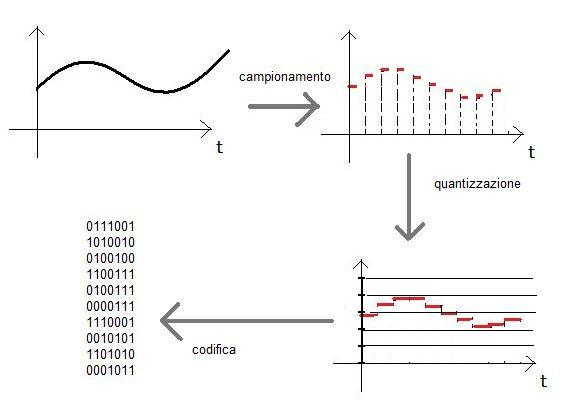
\includegraphics[width=0.5\textwidth]{./AnalogicoDigitale.jpg}
 % envelope.png: 220x138 pixel, 96dpi, 5.82x3.65 cm, bb=0 0 165 104
  \label{AnalogicoDigitale}
\caption{Discretizzazione di un suono da analogico a digitale}
\end{figure}

 
\subsubsection{Campionamento} 
Campionare l'audio significa creare una sequenza di campioni, ovvero i valori di un segnale audio in diversi momenti temporali quindi ogni campione memorizzato rappresenta un'ampiezza ad un dato istante. 
Viene chiamata frequenza di campionamento il numero di volte che viene campionato il segnale in un secondo.  \cite{elabA}.


Secondo il teorema di campionamento di Nyquist e Shannon in una conversione da analogico a digitale la minima frequenza di campionamento necessaria per evitare ambiguit\`a e perdita di informazione nella ricostruzione del segnale analogico originario, con larghezza di banda finita e nota, \`e pari al doppio della frequenza massima del suono che stiano convertendo.
Se non viene rispettato questo teorema, cio\`e si ha un sottocampionamento del segnale analogico nel dominio del tempo allora nel dominio delle frequenze si ha la produzione di frequenze non proprie del segnale originario (\textit{alias}) producendo cio\`e una distorsione del segnale originario divenuto ora non pi\`u fedele.

\begin{figure}[h]
 \centering
 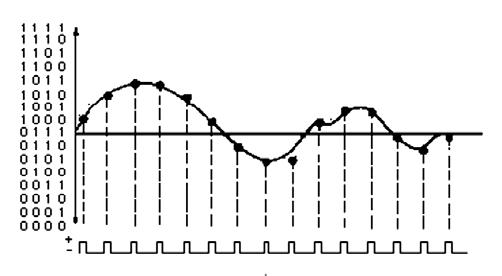
\includegraphics[width=0.7\textwidth]{./campionamento.jpg}
 % envelope.png: 220x138 pixel, 96dpi, 5.82x3.65 cm, bb=0 0 165 104
  \label{campionamento}
\caption{Campionamento e quantizzazione di un segnale continuo.}
\end{figure}


% Il segnale viene campionato e convertito in una sequenza di numeri, che vengono
% codificati con simboli. In generale, i segnali appartengono al mondo fisico e sono dovuti a fenomeni di
% tipo diverso. Ad esempio, il suono \`e dovuto alle variazioni della pressione dell’aria.
% Un sensore traduce la grandezza fisica in un segnale elettrico, che viene
% campionato e convertito in formato digitale.
% Al termine del processo di conversione, il segnale \`e stato trasformato in una
% sequenza di numeri che pu\`o essere elaborata, memorizzata o trasmessa.
% Il processo inverso consiste nel convertire i numeri in una sequenza di impulsi
% elettrici, che viene filtrata in modo da renderla simile al segnale originale. Il
% segnale elettrico cos\`i ottenuto viene inviato ad un trasduttore, che lo converte in
% un segnale fisico (suono).

\subsubsection{Quantizzazione}

Dopo il campionamento, la conversione analogico-digitale viene completata con la quantizzazione, che consiste nell'associare ad ogni campione un valore discreto.


Per ottenere ci\`o i valori possibili della grandezza in questione vengono innanzitutto limitati tra un massimo ed un minimo intorno a dei valori discreti preventivamente definiti, definendo cos\`i le relative regioni di decisione e la dinamica del quantizzatore stesso: in tal modo il valore analogico della grandezza originaria, 
in corrispondenza del valore campionato in ascissa, verr\`a ricondotto al pi\`u prossimo dei valori discreti preventivamente definiti tramite il processo di decisione.


Con la quantizzazione vengono per\`o introdotti degli errori detti \textit{errori di quantizzazione} pari alla differenza tra il valore quantizzato e il suo valore "reale" nel campo continuo. 
L'errore massimo possibile che potr\`a essere introdotto volta per volta sar\`a quindi pari alla met\`a dell'intervallo discreto discriminabile o regione di decisione. L'insieme di questi errori conduce al rumore di quantizzazione.


\section{Segnale}
In generale un segnale \`e una funzione di una o pi\`u variabili che contiene informazioni relative ad un fenomeno fisico. In questo caso ci interessano i segnali sonori che sono delle funzioni dell'ampiezza rispetto al tempo. 
I segnali possono essere classificati secondo le seguenti propriet\`a:
\begin{description}
  \item[Continuit\`a nel tempo]
    Un segnale pu\`o essere a tempo continuo o a tempo discreto a seconda che il dominio della funzione sia non numerabile o numerabile.
  \item[Continuit\`a nell'ampiezza]
    Un segnale pu\`o essere ad ampiezza continua oppure ad ampiezza discreta(o quantizzato) a seconda che l'immagine della funzione sia non numerabile o numerabile.
  \item[Periodicit\`a]
    Un segnale pu\`o essere periodico se esiste una quantit\`a $T$ nel dominio del tempo tale che per ogni tempo $t$ vale $s(T+t)=s(t)$. Se non vale questa propriet\`a allora il segnale \`e aperiodico. 
    Un segnale si dice quasi periodico se \`e composto dalla somma di segnali periodici con diverse frequenze che tra di loro stanno in rapporti non razionali. 
  \item[Determinatezza]
    Un segnale si dice determinato se \`e perfettamente noto e rappresentabile con una funzione che ne specifica l'andamento in ogni istante invece viene chiamato aleatorio se non \`e completamente noto a priori, ma pu\`o assumere un qualunque andamento entro una classe di funzioni specificata da alcune propriet\`a statistiche.
  \item[Stazionareit\`a]
    Un segnale stocastico, si dice stazionario se le sue propriet\`a statistiche non cambiano nel tempo, altrimenti si dice non stazionario.
\end{description}



\paragraph{Energia}
Dato un segnale $s(t)$ definiamo l'energia del segnale come:
\[
  E=\int_{-\infty}^{\infty} |s(t)|^{2}dt
\]
La definizione acquista significato fisico quando il segnale \`e reale, in tal caso, infatti supponendo che $s(t)$ rappresenti la tensione applicata o la corrente immessa ad una resistenza di $1Ohm$, questa \`e l'energia da essa dissipata. 
Definiamo la potenza media di un segnale continuo $s(t)$ il limite:
\[
  P=\frac{1}{2T} \lim_{T\rightarrow \infty} \int_{-T}^{T} |s(t)|^{2}dt
\]

Il segnale $s(t)$ \`e detto ad energia finita se $E$ \`e finito e diverso da zero. 
Il segnale \`e detto a potenza media finita se P \`e finito e diverso da zero. Si noti che se un segnale ha energia finita la sua potenza media \`e nulla e se un segnale ha potenza media finita la sua energia \`e infinita, pertanto le due classi sono disgiunte. 
Una classe importante di segnali a potenza media finita \`e costituita dai segnali periodici; in tal caso l'energia \`e finita e la potenza media coincide con quella calcolata in un periodo.



\section{Analisi nel dominio del tempo e nel dominio della frequenza}
\begin{comment}
dato un segnale infinito il suo contenuto in frequenza (il suo spettro) si pu\`o ottenere con una operazione matematica detta Integrale di Fourier. Il risultato dell'Integrale di Fourier di s(t) \`e una funzione a valori complessi S(ω) definita tra meno infinito e pi\`u infinito. I valori complessi portano con sé l'informazione relativa alla fase del segnale. 
Per esempio se si considera il segnale emesso da un sistema di altoparlanti multivia, spostando la posizione del tweeter cambia la fase del segnale e non il suo contenuto in frequenza, in altri termini il valore assoluto dell'Integrale di Fourier resta lo stesso. 
L'integrale di Fourier \`e reversibile, nel senso che a partire dal contenuto in frequenza si pu\`o costruire esattamente il segnale originale. 
Ricordo che stiamo parlando di operazioni matematiche svolte su segnali infiniti lavorando con quantit\`a senza errori, in altra parola segni di lapis su di un pezzo di carta ed esattamente va inteso in questo senso. 
Di solito quando si parla di spettro di un segnale si trascura la fase e si considera |S(ω)| (oppure se ci interessa la potenza espressa in decibel la quantit\`a 20 Log10 | S(ω)|). 
In entrambi i casi si pu\`o dimostrare che la parte positiva e la parte negativa delle funzioni risultanti sono specularmente uguali e quindi di solito se ne disegna solo la parte positiva. 
Con questa semplificazione per\`o si perde la reversibilit\`a e quello che resta \`e solo una misura effettuata sul segnale, priva dell'informazione completa. Per comprendere appiano il significato dell'integrale di Fourier sono necessari alcuni preliminari matematici.
\end{comment}
I principali metodi di analisi del segnale possono essere riassunti nei concetti di analisi nel dominio del tempo e analisi nel dominio della frequenza. 
\`E importante osservare che questi due modi di affrontare un problema sono tra loro intercambiabili, nel senso che, sotto opportune condizioni, nessuna informazione viene persa nel passare da un dominio all'altro. 
Il vantaggio che deriva dall'introduzione dei due domini \`e la possibilit\`a di cambiare la prospettiva con la quale si osserva un dato fenomeno. 
In questo modo un problema che appare di difficile soluzione in un dominio pu\`o risultare molto pi\`u semplice nell'altro \cite{DomTF}.

\paragraph{Analisi nel dominio del tempo}
Questa forma di rappresentazione \`e quella che ci \`e maggiormente familiare, in essa appaiono le variazioni subite dal segnale al trascorrere del tempo. 
Lo strumento pi\`u frequentemente usato e che opera notoriamente nel dominio del tempo \`e l'oscilloscopio.

\paragraph{Analisi nel dominio della frequenza}

Invece di analizzare le variazioni del segnale al passare del tempo, mostra come e quanto un segnale si suddivide o \`e distribuito nelle varie bande di frequenza, definite all'interno di un dato range. 
Viene chiamata analisi spettrale e lo strumento matematico che consente di trasferire lo studio dei segnali e dei sistemi dal dominio del tempo al dominio della frequenza \`e la trasformata di Fourier.

%
\begin{figure}[htbp]
\centering
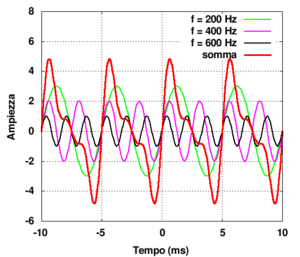
\includegraphics[width=0.4\textwidth]{./DominioTempo.png}%
\qquad\qquad
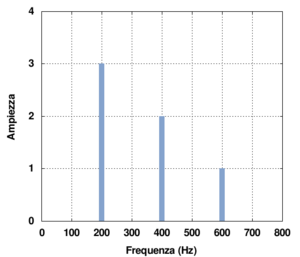
\includegraphics[width=0.4\textwidth]{./DominioFrequenze.png}
\caption{Esempi di grafici nel dominio del tempo e nel dominio delle frequenze \cite{IDOMTF}}
\end{figure}